\section{Was ist eigentlich Docker?}\label{sec:docker-runtime}
\subsection{Funktionsweise}

\begin{frame}
    \slidehead
    \vspace{-1em}
    \Large
    \centering
    \includesvg[height = 3em]{../pictures/docker_engine}
    \\
    Enthält:
    \begin{itemize}
        \item Container, als Einheiten
        \item Runtime, die die Container ausführt
    \end{itemize}
\end{frame}

\section{Docker}

\subsection{Was ist ein Container?}

\begin{frame}
    \slidehead
    \vspace{-1em}
    \Large
    \centering
    Eine Einheit bestehend aus:
    \begin{itemize}
        \item Einem ausführbarem \textbf{Docker-Image}
        \item Netzwerkeinstellungen wie \textbf{Port-Zuteilungen}
        \item Zugeteilten \textbf{Volumes}
        \item Eingerichteten \textbf{Mounts}
        \item und vielen weiteren Konfigurationen
    \end{itemize}
\end{frame}


%Docker-Image
\subsection{Docker-Image}

\begin{frame}
    \slidehead
    \vspace{-1em}
    \Large
    \centering
    Ein Image besteht aus folgenden Komponenten:
    \vspace{1em}
    \begin{itemize}
        \item Executabe
        \item Dependencies
        \item Default Configurations
    \end{itemize}
    \vspace{1em}
    Ein Image wird durch eine \textbf{Dockerfile} erstellt (später mehr dazu)
\end{frame}

%VMs-VS Docker

\subsection{VMs vs Docker}

\begin{frame}
    \slidehead
    \Large
    Docker benutzt die cgroups aus der Linux-Kernel um die einzelnen Prozesse aus dem Image zum Hostsystem
    und den anderen Containern zu isolieren. \\
    Zur isolierung des Netzes wird ein virtueller Netzwerkadapter erstellt, der in den Container gebunden wird.
\end{frame}

\begin{frame}
    \slidehead
    \vspace{-1em}
    \Large
    \centering
    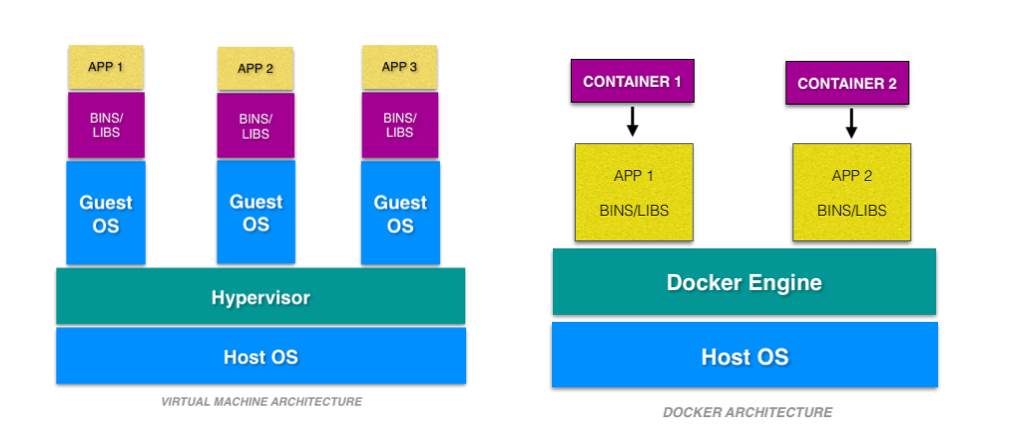
\includegraphics[height = 10em]{../pictures/docker-vs-vm.png}
\end{frame}

\begin{frame}
    \slidehead
    \Large
    \centering
    Vorteile der Container-Architektur:
    \vspace{1em}
    \begin{itemize}
        \item Weniger Resourcenverbrauch durch: \\
              - Mitbenutzung des Host-Kernels \\
              - Fehlen des Betriebssystemes des Gastes
        \item Dadurch können Container auch schneller deployt werden
        \item Ist aber funktional ähnlich zu VMs mit Mounts / Images / Ports
    \end{itemize}
\end{frame}

\subsection{Volumes und Mounts}
\begin{frame}
    \slidehead
    \Large
    Um persistenten Speicher für die Container zu ermöglichen, muss entweder ein Volume spezifiziert werden,
    welches von der Docker-Runtime verwaltet wird. \\
    Alternativ kann auch eine Datei / ein Ordner aus dem Hostsystem in den Container eingebunden (gemountet werden).\\
    Dies kann in der \textbf{docker-compose} geschehen.
\end{frame}

\subsection{Portfreigaben}
\begin{frame}
    \slidehead
    \Large
    Dadurch dass Container ihr eigenes Netz haben, müssen falls Services auf Ports anfragbar sein sollen, diese in den
    Container durchgeleitet werden. Dabei kann ein beliebiger Port vom Hostsystem auf einen beliebigen Port im Container
    gemappt werden. Dies kann auch in der \textbf{docker-compose} geschehen.


\end{frame}
